\section[Системное описание предметной области и постановка задачи]{%
  СИСТЕМНОЕ ОПИСАНИЕ ПРЕДМЕТНОЙ \\
  ОБЛАСТИ И ПОСТАНОВКА ЗАДАЧИ
}\label{sec:spec}

% Выбор программной платформы

\subsection{Выбор программной платформы}

Для того, чтобы правильным образом выбрать программную платформу, обратимся к
общей тенденции развития рынка персональных компьютеров и мобильных устройств.

Начиная с 2012 года мировой рынок ПЭВМ начинает показывать спад:
в третьем квартале этого года наблюдается снижение объёма
поставок техники на 8,6\% по сравнению с аналогичным периодом
2011 года, по данным международной исследовательской компании IDC, при том,
что ранее аналитики этой компании прогнозировали понижение только на 3,8\%.

Спад мирового рынка персональных компьютеров продолжается и сегодня: в январе 2016
года аналитики IDC сообщили об обвале мирового рынка этих устройств.
Объём рынка ПЭВМ в 2015 году впервые за семь лет оказался ниже 300 млн единиц,
а спад --- рекордным. Согласно расчетам экспертов, в 2015 году вендоры отгрузили
по всему миру 276,2 млн десктопов и ноутбуков, что на 10,4\% меньше, чем годом ранее.
Столь сильного падения на рынке не было никогда.
Прежде сильнейший регресс (на 9,8\%) произошел в 2013 году, а поставки ПК последний
раз падали ниже 300 млн устройств лишь в 2008 году,
отмечается в исследовании~\cite{computers_world_market}.

Однако на рынке мобильных устройств, наооборот, наблюдается стремительный рост.
Толчком к этому росту послужил представленный 9 января 2007 года на конференции
Macworld Conference \& Expo в Сан-Франциско первый iPhone. В своём выступлении
Стив Джобс сказал: «Сегодня Apple собирается переизобрести телефон>>~\cite{apple_reinvent_phone}.

Стоит отметить, что первоначальные отзывы на новый iPhone были крайне противоречивыми.
Так, некоторые журналисты оставляли следующие сообщения после презентации продукта:
<<кнопки на сенсорном экране? Плохая идея. Это не сработает>>,
<<похоже, ребята, никто из вас не осознает, насколько неудачна идея сенсорного
экрана в телефоне. Я уже предвижу ряд очевидных и серьезных проблем>>.
Однако, с течением времени можно действительно сказать, что Apple переизобрела телефон.
В итоге с 2007 года производители всех мобильных устройств
стали стремиться к новому форм-фактору: наличие большого мультитач экрана
с возможностью обработки пользовательских жестов.

В подтверждение роста рынка мобильных устройств можно привести график сравнения
продаж iOS устройств, которые составляют около 12\% рынка всех смартфонов,
с устройствами под управлением OC Windows, представленный
на рисунке~\ref{fig:ios_windows_compare}.

\begin{figure}[h!]
  \centering
  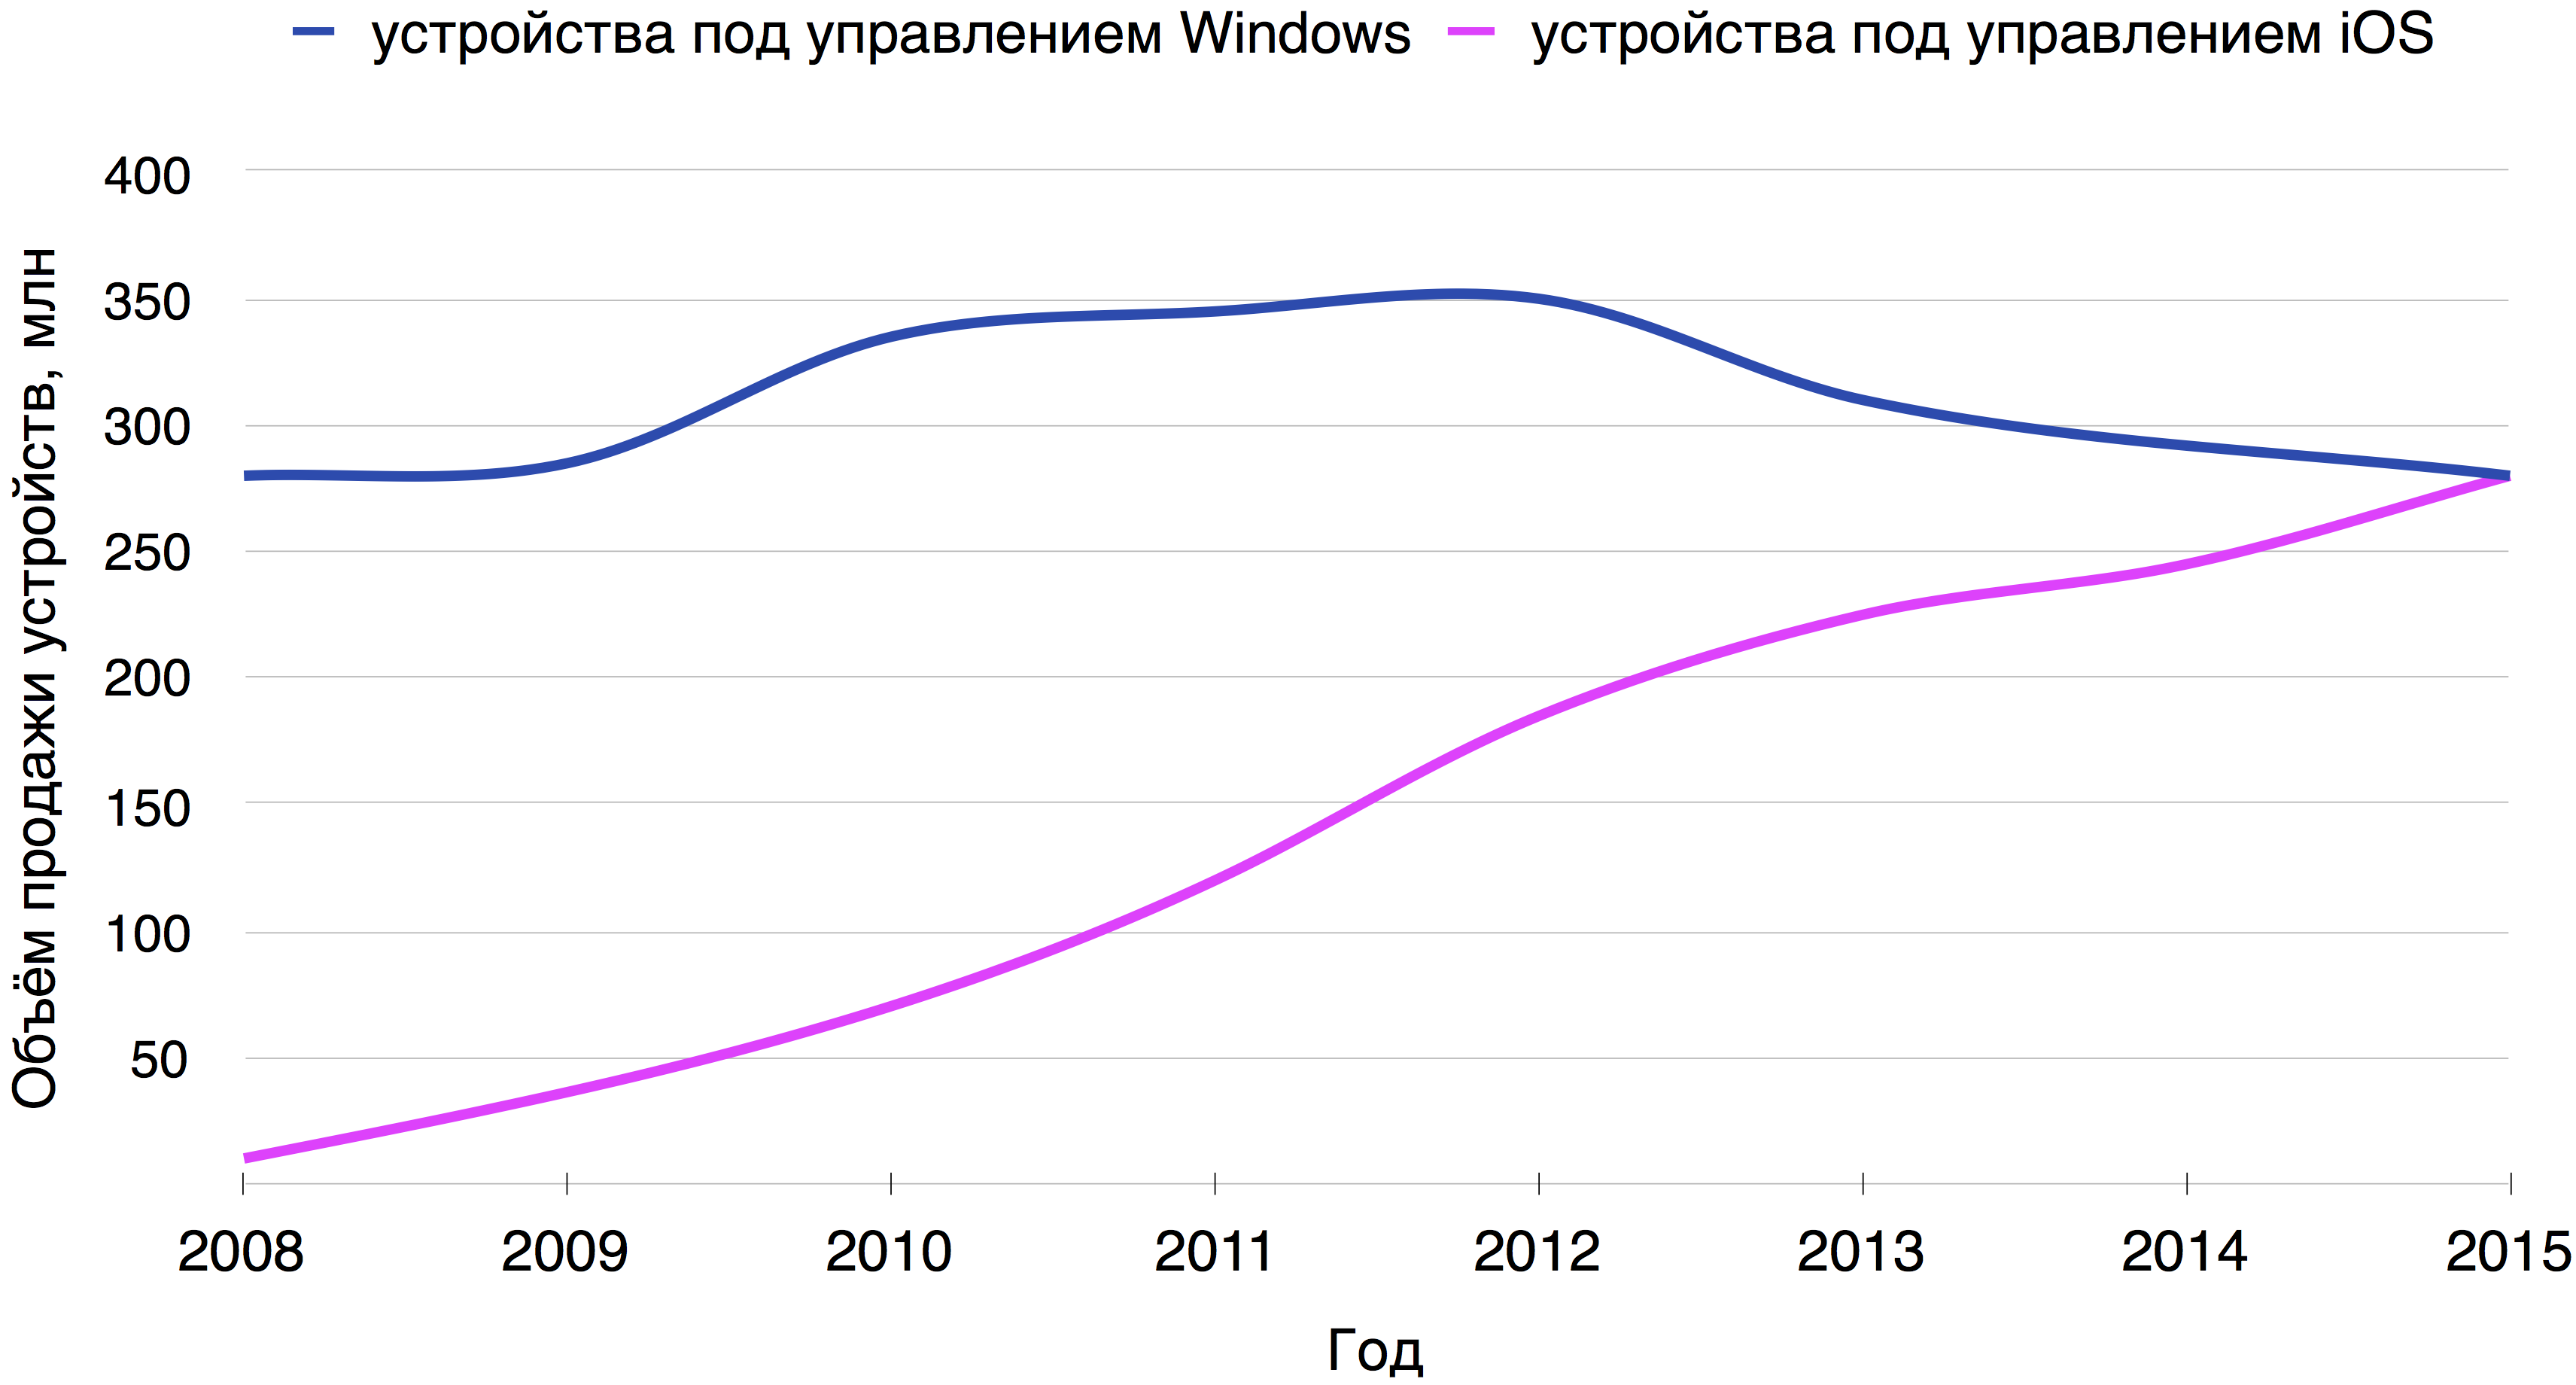
\includegraphics[width=150mm]{fig/ios_windows_compare}
  \caption{Сравнение объёма продаж устройств \\ под управлением iOS и Windows}
  \label{fig:ios_windows_compare}
\end{figure}

Из приведенного рисунка видно, что объём продаж устройств под управлением
iOS превысил продажи устройств под управлением OC Windows в июне 2015 года, а
годовые объёмы продаж устройств на Android превысили ПК ещё в марте 2012 года.
Количество действующих персональных компьютеров на платформе Windows оценивается
в 1,5 млрд устройств, объем работающих устройств на Android уже превысил этот
показатель, а iOS вполне может преодолеть аналогичный рубеж.

Мобильные устройства становятся удобнее для решения повседневных задач,
чем компьютеры. Этому служат следующие факторы:
\begin{itemize}
  \item развитие сети интернет-вещания 3G, LTE;
  \item различные форм-факторы устройств;
  \item наличие рынка мобильных приложений;
  \item активное взаимодействие устройства с пользователем с использованием сервисов
    геолокации, push- и локальных уведомлений.
\end{itemize}

Нативные приложения требуют установки и разрабатываются индивидуально
под мобильные платформы с использованием библиотек, предлагаемых
компанией-производителем операционной системы. Это позволяет выдерживать все
мобильные приложения в стиле операционной системы. Уникальность приложениям
придают дизайнерские решения элементов интерфейса, а также внутренняя реализация
бизнес-логики.
В отличие от Web-приложений, мобильные приложения, благодаря тесному
взаимодействию с операционной системой устройства, позволяют с наименьшими
трудозатратами использовать встроенную камеру, микрофон, акселерометр,
плеер и прочие элементы девайса.

Стоит отметить, что мобильная операционная система iOS по популярности
сильно уступает Android.
Между тем, главным преимуществом компании Apple является
состоятельность её аудитории. При маленьком объёме рынка (около 12\%),
на устройства iOS приходится половина всех доходов
от продажи приложений --- \$6,4 млрд в год.
Кроме того, устройства Apple не так просто взломать.
Это еще одна причина высокой покупательской способности на платформе.

По данным на февраль 2016 года большинство iOS устройств~(более~77\%) используют
последнюю версию операционной системы от Apple, тогда как только 7,5\%
устройств на Android обновились до последней версии Android Marshmallow (данные
на май 2016 года), хотя загрузка образов этой операционной системы стала
возможна ещё осенью 2015 года.
Диаграммы использования различных версий операционных систем iOS и Android
представлены на рисунках~\ref{fig:android_versions}--\ref{fig:ios_versions}.

\begin{figure}[h]
  \begin{center}
    \begin{minipage}[h]{0.47\linewidth}
      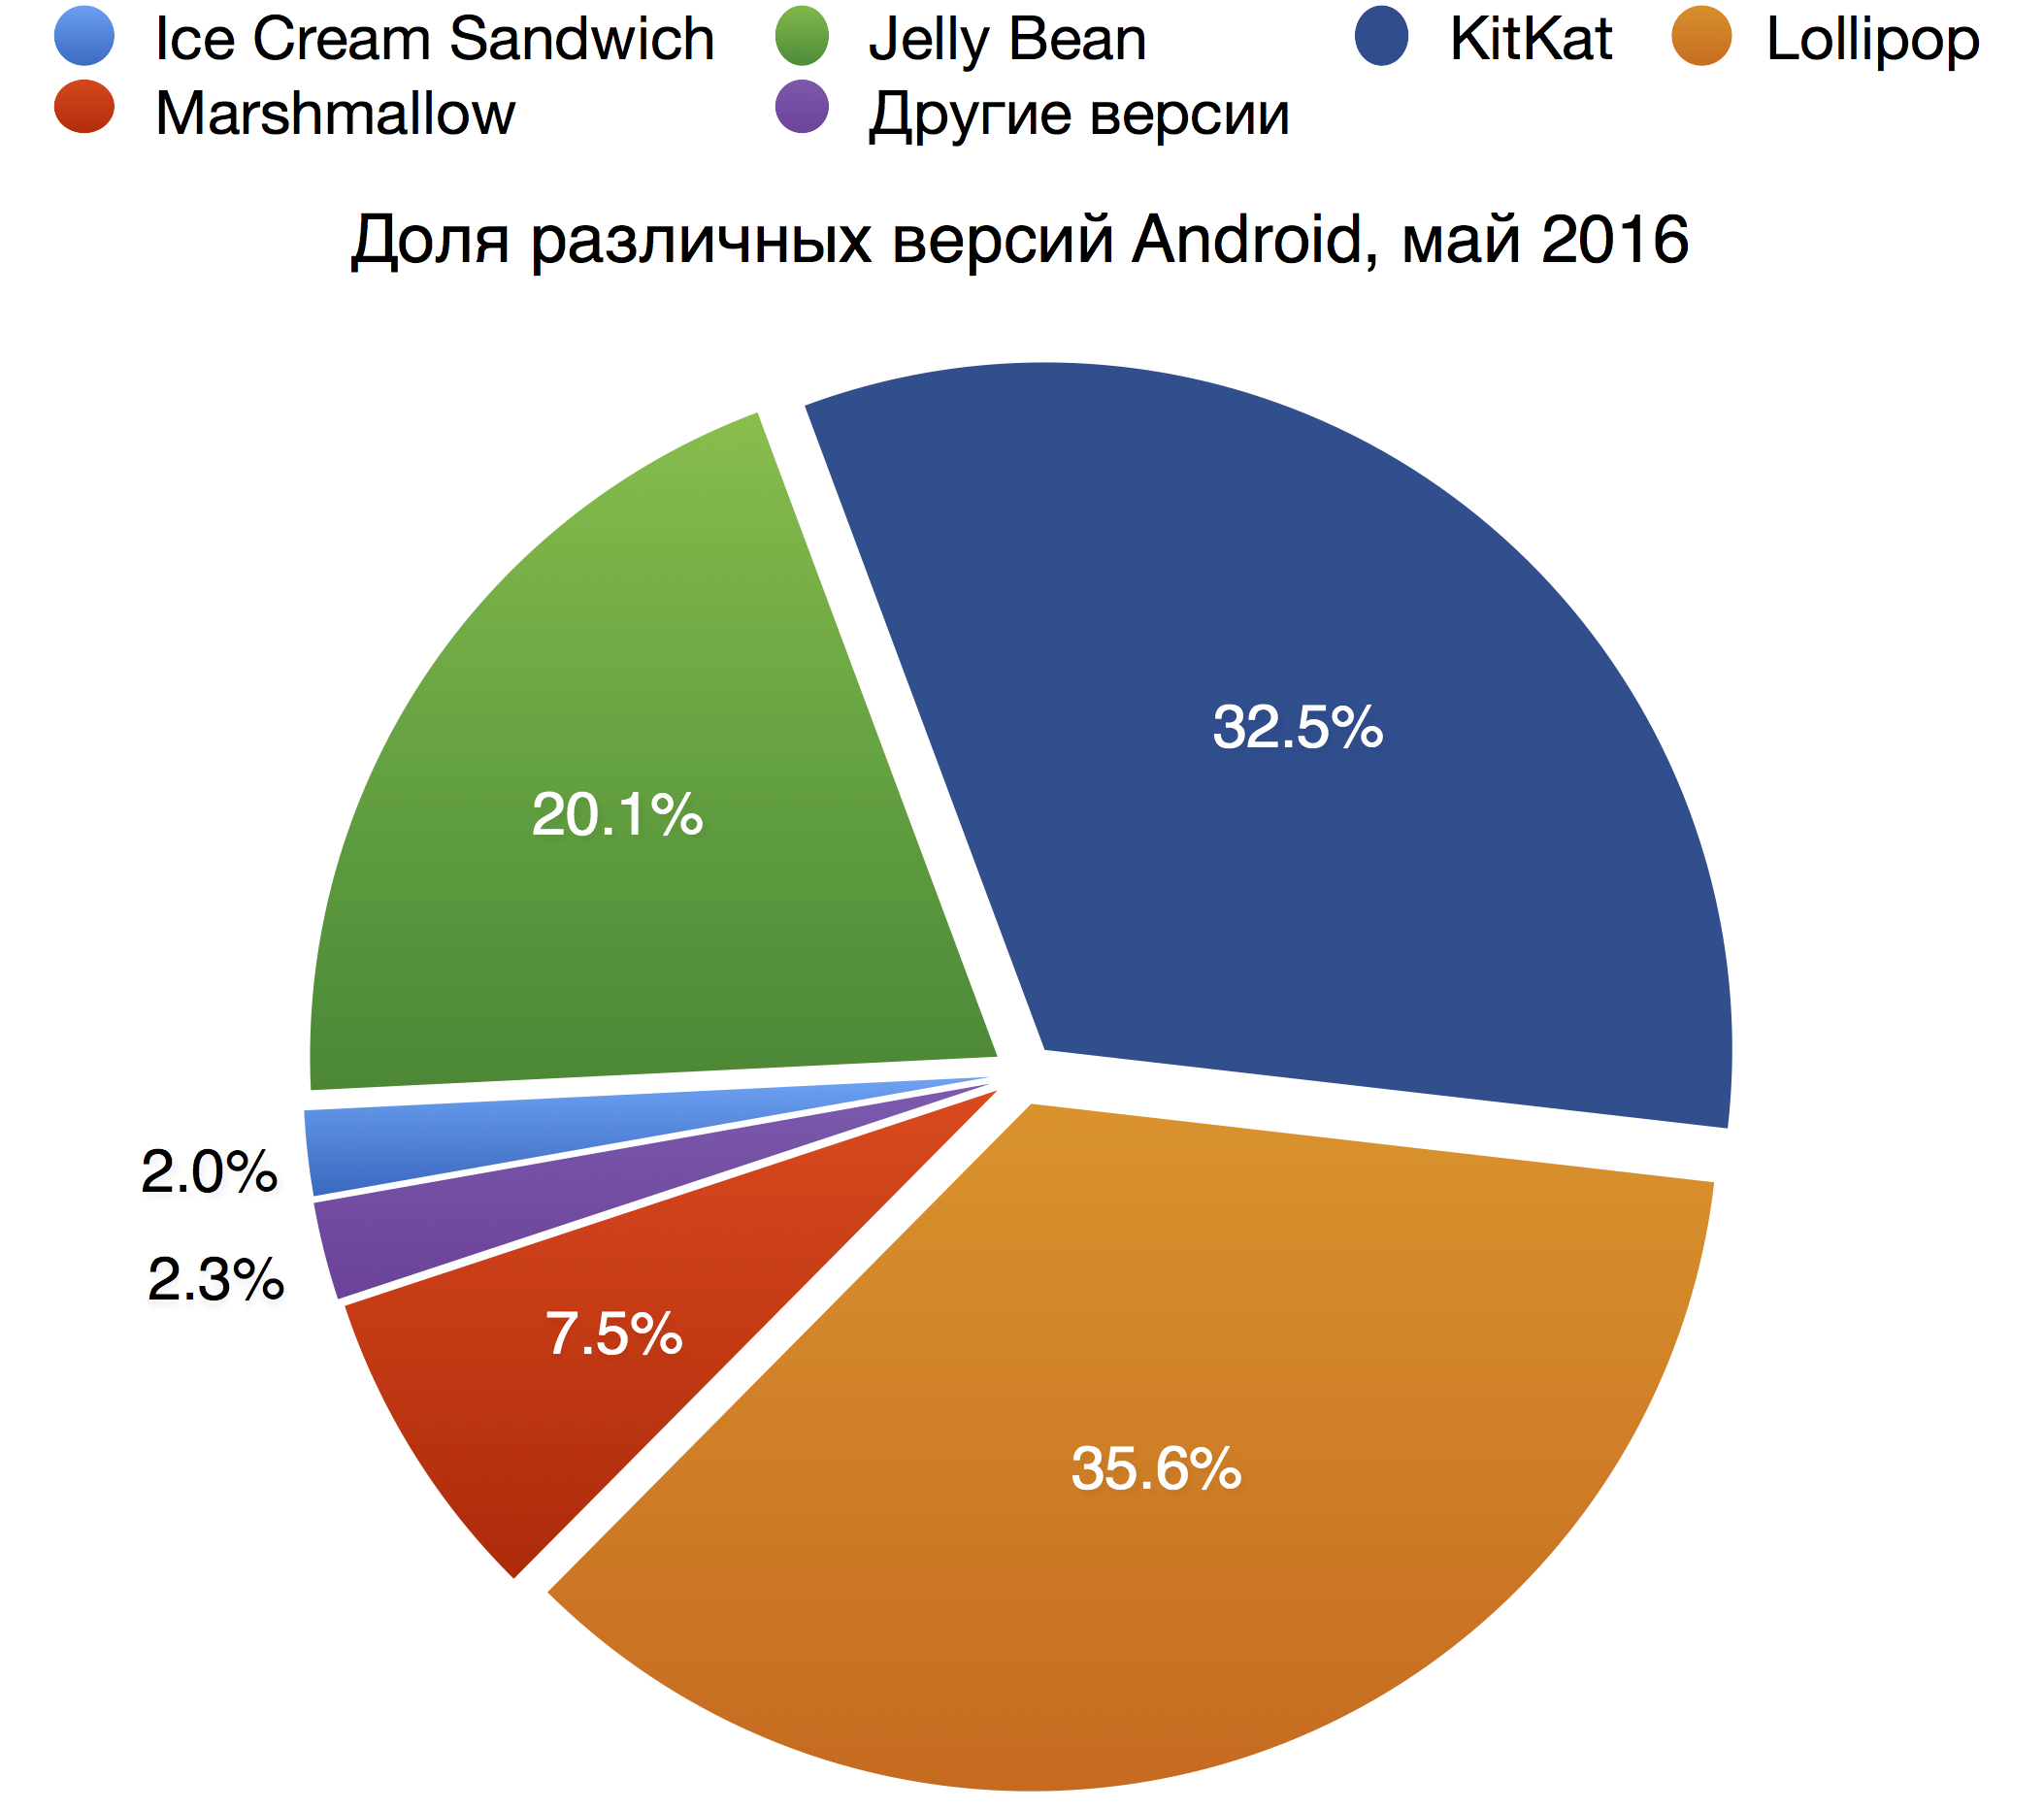
\includegraphics[width=1\linewidth]{fig/android_versions}
      \caption{Доля устройств под управлением различных версий Android}
      \label{fig:android_versions}
    \end{minipage}
    \hfill
    \begin{minipage}[h]{0.47\linewidth}
      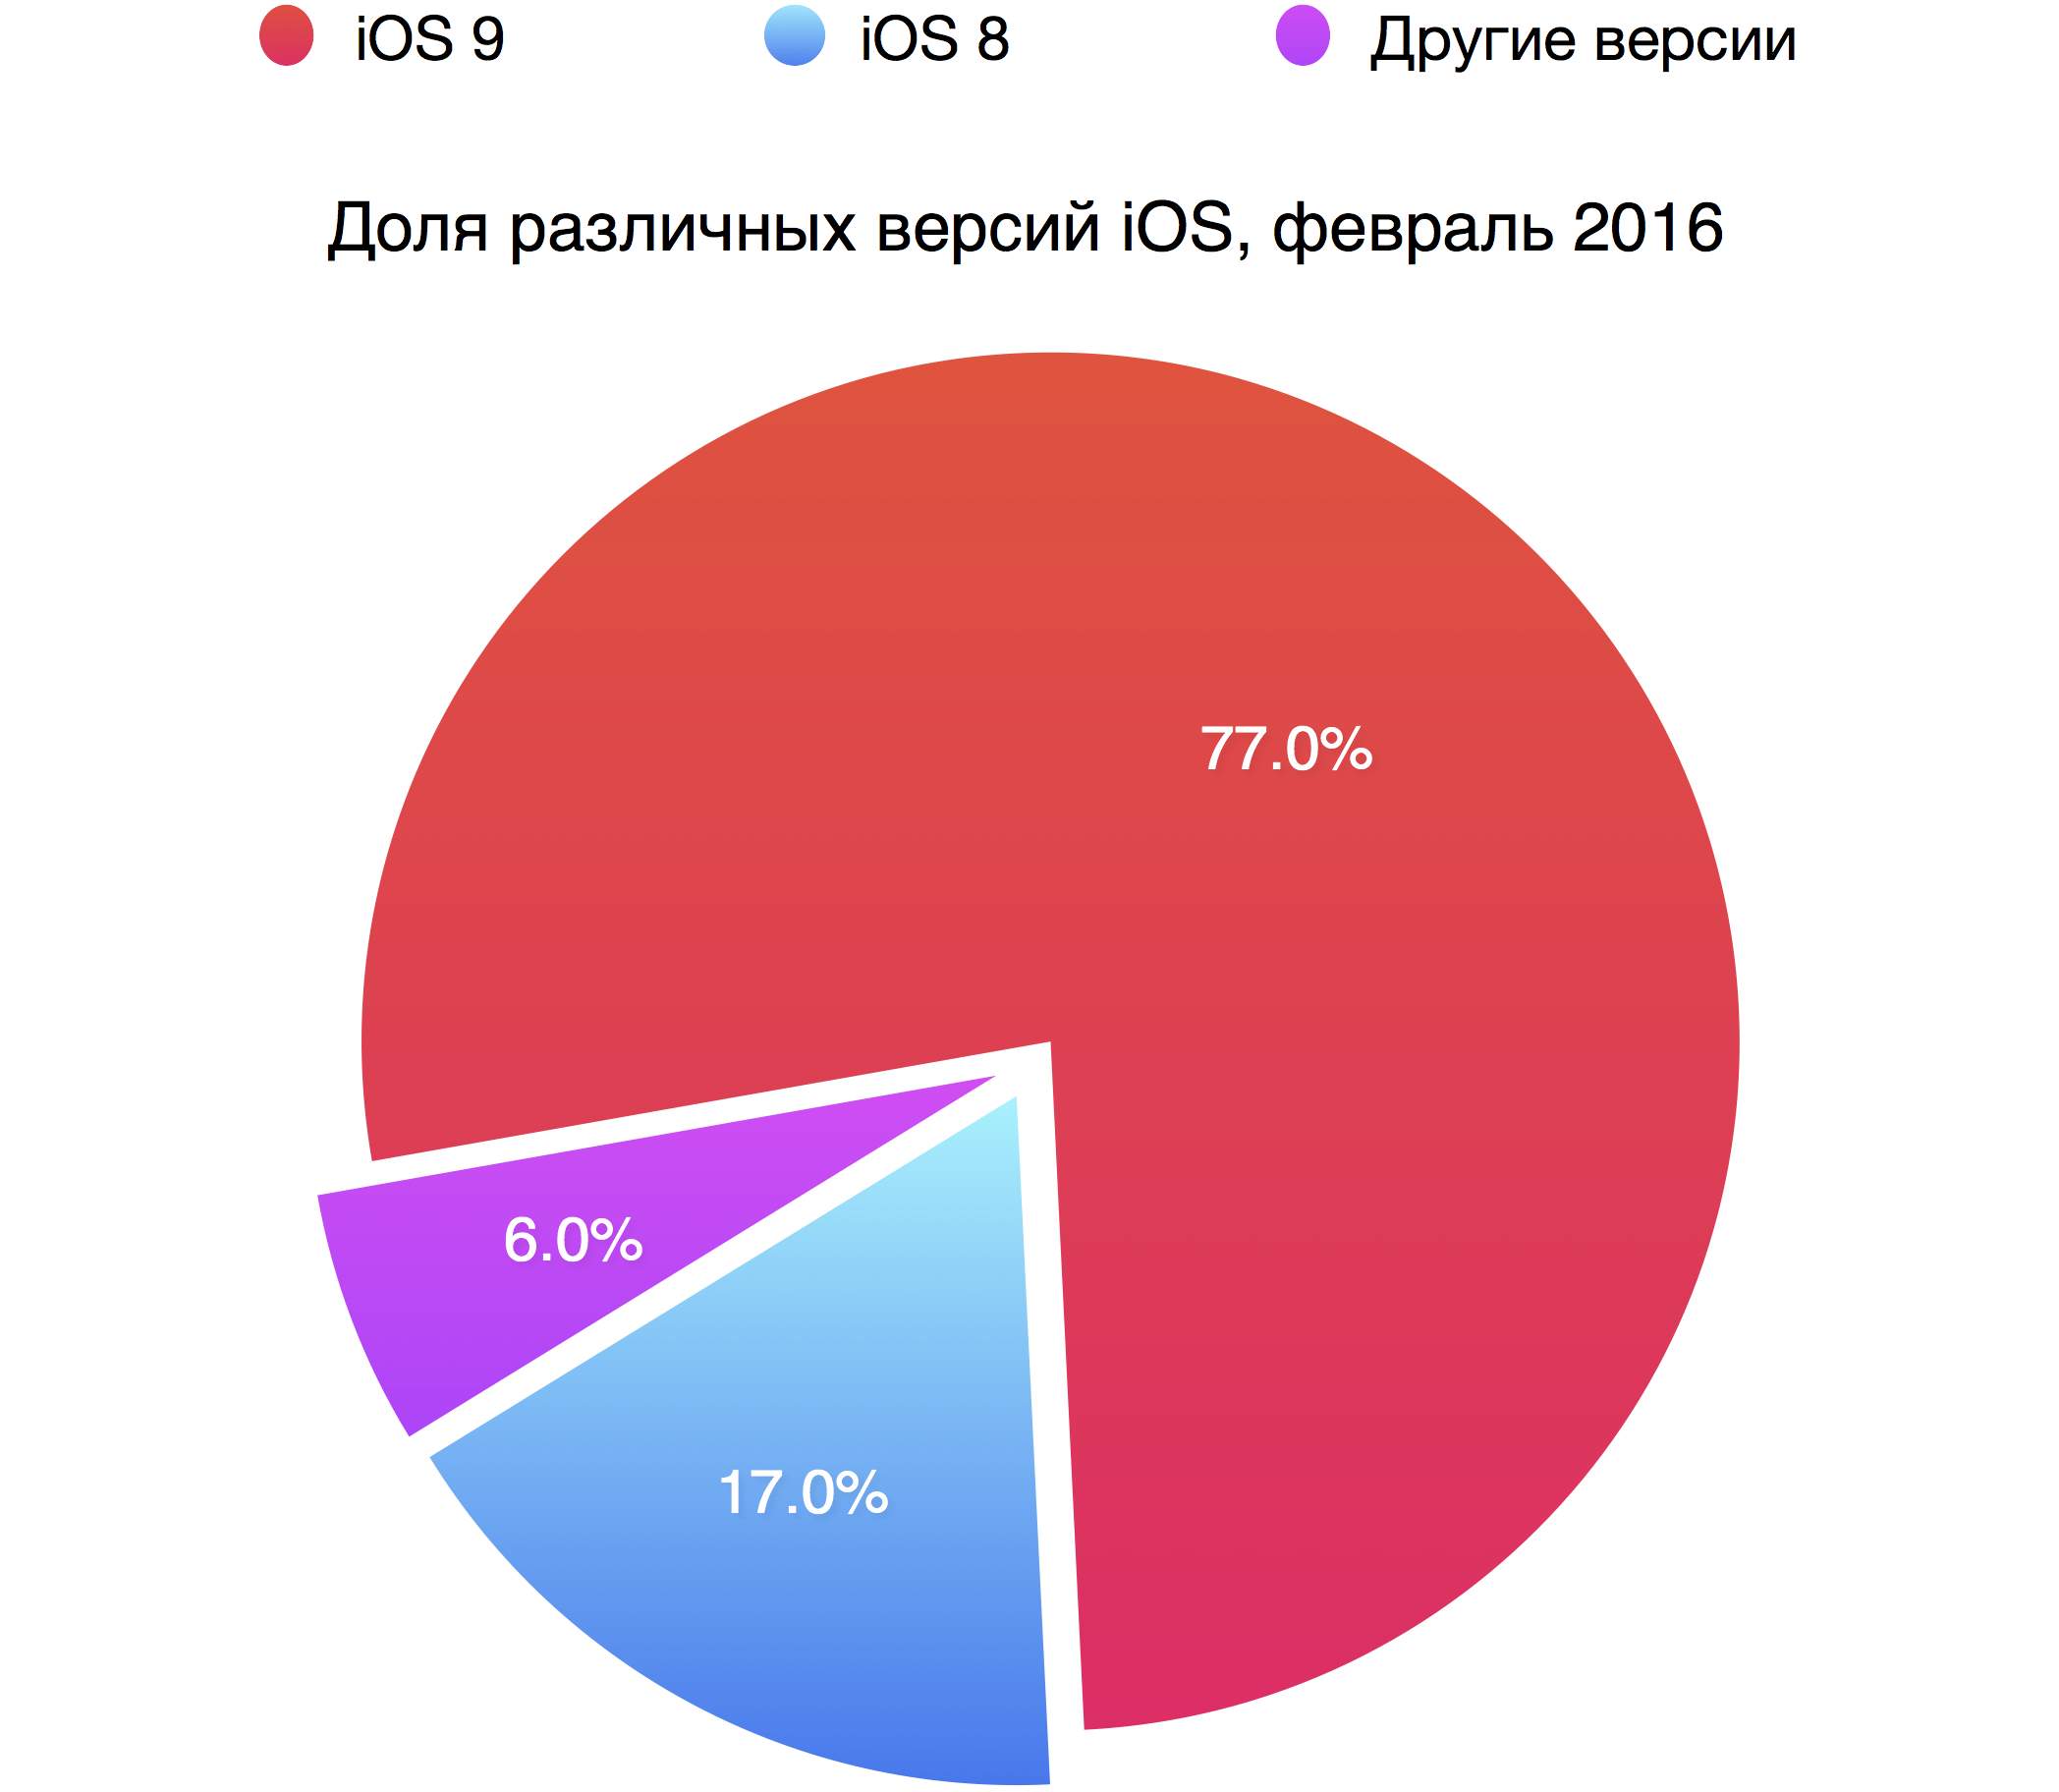
\includegraphics[width=1\linewidth]{fig/ios_versions}
      \caption{Доля устройств под управлением различных версий iOS}
      \label{fig:ios_versions}
    \end{minipage}
  \end{center}
\end{figure}

Сами разработчики мобильных приложений отдают предпочтение платформе Apple.
Отчасти это связано с тем, что при проектировании нужно учитывать всего
несколько форматов дисплеев, и как правило, в поддержке предыдущих
версий операционных систем практически нет необходимости.
Ещё одним фактором в пользу Apple является состоятельность её аудитории,
обеспечивая высокую эффективность монетизации приложений~\cite{ios_android_compare}.


% Выводы по подразделу

Опираясь на то, что целевым назначением разрабатываемого программного модуля
является предоставление пользователю актуальной финансовой информации,
то целесообразным является разработать этот модуль в форм-факторе мобильного
приложения, потому что именно мобильное приложение позволяет в кратчайшие сроки
и с минимальными трудозатратами передать пользователю необходимую финансовую
информацию.
Учитывая перечисленные выше достоинства операционной системы iOS, в качестве
целевой мобильной платформы выберем операционную систему iOS,
целевое устройство --- iPhone.

В 2014 году компания Apple представила новый язык программирования Swift,
который позволяет создавать более безопасные и быстрые приложения, в сравнении
с его предшественником Objective-C.
Начиная с декабря 2015 года, Swift является языком с открытым исходным кодом.
Таким образом, разработчики со всего мира могут вносить свой вклад
в этот язык программирования и делать его доступным на новых платформах.
Эффективность и простота Swift дают молодым программистам стимулы к обучению,
к тому же теперь они могут распространять свои идеи повсюду:
от мобильных устройств до облачных систем~\cite{swift_becomes_open_source}.


% Сравнительный анализ существующих аналогов

\subsection{Сравнительный анализ существующих аналогов}

Рассмотрим наиболее популярные iOS приложения, позволяющие просматривать
информацию о курсах валют. Для этого воспользуемся магазином приложений от Apple,
введя в строке поиска запрос <<Курсы валют>>. В результате на выбор
пользователю будет представлено более десятка мобильных приложений в данной
категории. Учитывая то, что в App Store используется достаточно
простой алгоритм формирования списка приложений, основанный прежде всего на
количестве скачиваний, можно утверждать, что первые приложения из этого списка
являются наиболее популярными.

Рассмотрим первые пять приложений из этого списка, указав название приложения
в кавычках, разработчика в круглых скобках:
\begin{itemize}
  \item <<Курсы валют в Минске>> (Alex L);
  \item <<Курсы валют, банкоматы, обменники>> (Alex L);
  \item <<Финансы TUT.BY: курсы валют, конвертер>> (TUT.BY);
  \item <<Онлайнер - новости, курсы валют>> (Orangesoft LLC);
  \item <<Курс Валют Беларусь>> (Mobinovo).
\end{itemize}

Все приведенные приложения распространяются бесплатно, и только некоторые из
них включают <<встроенные покупки>>, то есть возможность расширения
функциональности приложения за счёт некоторого вознаграждения.

Для сравнения приложений будем использовать ряд критериев, которые условно
можно разделить на две группы: критерии функциональности и критерии удобства
использования.

Приложение <<Курс Валют Беларусь>> можно убрать из рассмотрения, так как оно
закрывается сразу после открытия (приложение принудительно завершается
стандартным обработчиком ошибок).

Приведём критерии функциональности:
\begin{itemize}
  \item возможность отображения курсов валют в коммерческих банках;
  \item возможность отображения курсов валют, установленных национальным
    банком Республики Беларусь;
  \item наличие информации об отделениях банка;
  \item возможность отображения курсов валют в отделениях;
  \item возможность отображения отделения (банка) на карте;
  \item возможность поиска ближайших отделений (банков);
  \item отображение курсов валют в регионах;
  \item возможность отправки Push-уведомлений;
  \item возможность добавления отделений (банков)
    в избранное или закладки.
\end{itemize}

Критерии функциональности составлены с учётом основных возможностей
мобильных устройств, предоставляемой информации веб-ресурсами (API),
а также на основе изучения финансов порталов, предоставляющих пользователю
информацию о курсах валют.

Приведём критерии удобства использования:
\begin{itemize}
  \item стабильность работы приложения;
  \item простота восприятия информации;
  \item актуальность предоставляемой информации;
  \item дизайн (соответствие последней версии iOS);
  \item наличие рекламы;
\end{itemize}

Критерии удобства использования приложения сформированы на основе личного опыта
использования устройств под управлением операционной системы от Apple, а также
документа, содержащего рекомендации по разработке iOS приложений~---
iOS Human Interface Guidelines~\cite{ios_hig}.

Для получения максимально объективной оценки сравнительного анализа в перечень
критериев не будем включать какие-либо конкретные составляющие дизайна, такие как
шрифт, размер текста или основную цветовую схему приложения. Вместо этого,
постараемся убедится в том, что рассматриваемые приложения
соответствует рекомендациям документа iOS Human Interface Guidelines.

Произведем сравнение существующих аналогов по приведенным критериям. Для удобства
восприятия полученной информации, представим результаты сравнения в виде таблиц.
Результат сравнения по критериям функциональности представлен
в таблице~\ref{tbl:functionality_compare}.

\begin{table} [h!]
  \caption{
    Сравнение аналогов по критериям функциональности
  }\label{tbl:functionality_compare}
    \begin{tabular}{| m{8.5cm} | c | c | c | c |}
      \hline
      \parbox{7cm}{
        Критерий сравнения
      }
      & \rotatebox[origin=c]{90}{
          \parbox{4.2cm}{
            Курсы валют \\ в Минске
          }
        }
      & \rotatebox[origin=c]{90}{
          \parbox{4.2cm}{
            Курсы валют, \\ банкоматы, \\ обменники
          }
        }
      & \rotatebox[origin=c]{90}{
          \parbox{4.2cm}{
            Финансы TUT.BY: \\ курсы валют, \\ конвертер
          }
        }
      & \rotatebox[origin=c]{90}{
          \parbox{4.2cm}{
            Онлайнер -- \\ новости, \\ курсы валют
          }
        }
      \\
      \hline

      Отображение курсов валют \par в коммерческих банках
      & +
      & +
      & +
      & + \\
      \hline

      Отображение курсов валют \par национального банка РБ
      & +
      & +
      & +
      & + \\
      \hline

      Информация об отделениях банка
      & +
      & +
      & +
      & + \\
      \hline

      Отображение курсов валют \par в конкретных отделениях
      & -
      & -
      & +
      & + \\
      \hline

      Отображения отделений (банков) \par на карте
      & -
      & +
      & +
      & + \\
      \hline

      Поиск ближайших отделений \par (банков)
      & -
      & +
      & +
      & - \\
      \hline

      Отображение курсов валют \par в регионах
      & -
      & +
      & +
      & -  \\
      \hline

      Наличие Push-уведомлений
      & -
      & +
      & -
      & -  \\
      \hline

      Добавления отделений (банков) \par в избранное или закладки
      & -
      & +
      & -
      & -  \\
      \hline

    \end{tabular}
\end{table}

\newpage

Результат сравнения по критериям удобства использования представлен
в таблице~\ref{tbl:ux_compare}.

\begin{table} [h!]
  \caption{
    Сравнение аналогов по критериям удобства использования
  }\label{tbl:ux_compare}
    \begin{tabular}{| m{8.5cm} | c | c | c | c |}
      \hline
      \parbox{7cm}{
        Критерий сравнения
      }
      & \rotatebox[origin=c]{90}{
          \parbox{4.2cm}{
            Курсы валют \\ в Минске
          }
        }
      & \rotatebox[origin=c]{90}{
          \parbox{4.2cm}{
            Курсы валют, \\ банкоматы, \\ обменники
          }
        }
      & \rotatebox[origin=c]{90}{
          \parbox{4.2cm}{
            Финансы TUT.BY: \\ курсы валют, \\ конвертер
          }
        }
      & \rotatebox[origin=c]{90}{
          \parbox{4.2cm}{
            Онлайнер -- \\ новости, \\ курсы валют
          }
        }
      \\
      \hline

      Стабильность работы приложения
      & +
      & +
      & +
      & + \\
      \hline

      Простота восприятия информации
      & +
      & -
      & -
      & + \\
      \hline

      Актуальность предоставляемой \par информации
      & +
      & +
      & +
      & + \\
      \hline

      Дизайн (соответствие последней \par версии iOS 9)
      & +
      & -
      & +
      & + \\
      \hline

      Отсутствие рекламы
      & -
      & -
      & +
      & + \\
      \hline

    \end{tabular}
\end{table}

Из приведенной сравнительной характеристики видно, что каждое из приложений
обладает рядом достоинств, но вместе с тем, имеет и ряд недостатков.

Например, приложение <<Онлайнер -- новости, курсы валют>>, несмотря на высокие
показатели по критериям <<удобство использования>>, является, в первую очередь,
новостным приложением, и курсы валют предоставляет в качестве дополнительного сервиса.

В то же время приложение <<Курсы валют в Минске>>, несмотря на достаточно
ограниченную функциональность, является наиболее простыми в использовании, так как
предоставляет всю информацию о курсах валют на одном экране. Однако, если
пользователю требуется найти отделение банка на карте, то понадобится открывать
стороннее приложение, которое, в свою очередь, является очень перегруженным.

В результате сравнения можно выделить приложение <<Курсы валют
в Минске>> и <<Финансы TUT.BY: курсы валют, конвертер>>. Оба эти приложения
соответствуют рекомендациям Apple по разработке мобильных приложений,
предоставляют актуальную информацию, но при этом обладают
разной функциональностью.
Снимки главных экранов приведенных приложений приведены на рисунке~\ref{fig:tutby_exchanges_minsk_screenshots}.

\begin{figure} [h]
  \begin{minipage} [h] {0.49\linewidth}
    \center{
      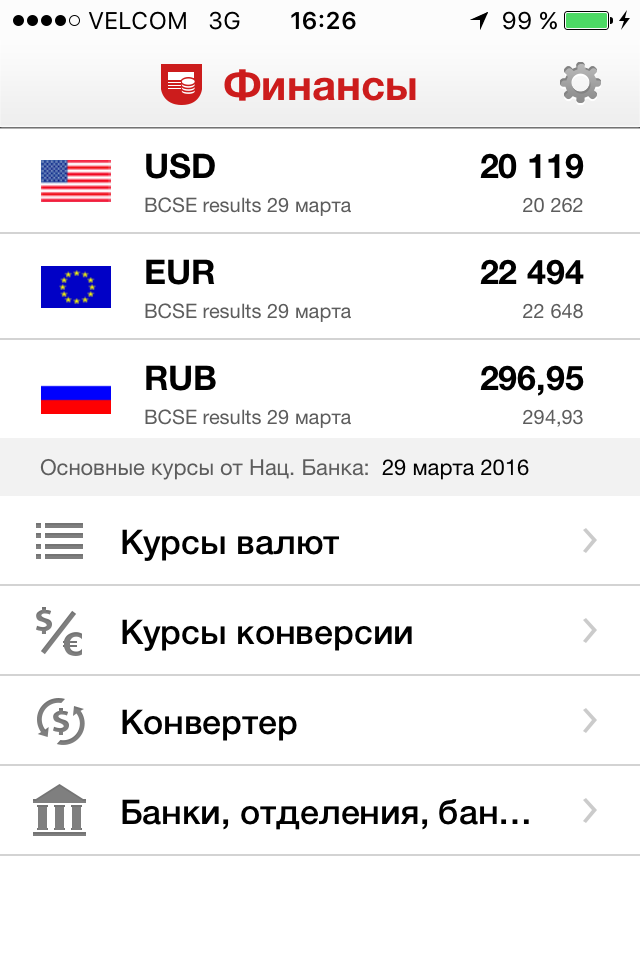
\includegraphics[width=0.9\linewidth]{fig/tut_by_screen}
    }
  \end{minipage}
  \hfill
  \begin{minipage} [h] {0.49\linewidth}
    \center{
      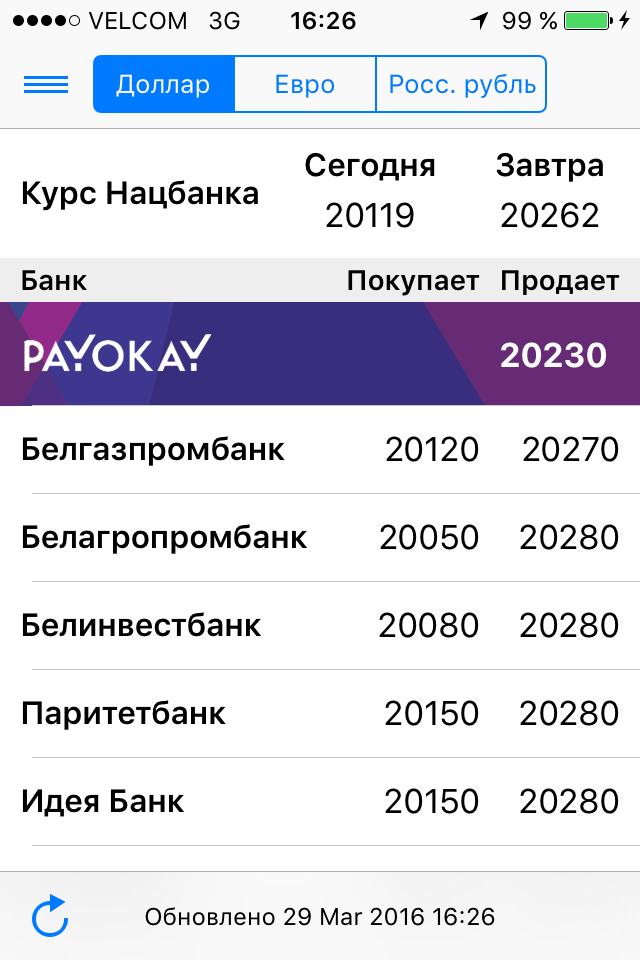
\includegraphics[width=0.9\linewidth]{fig/exchanges_minsk_screen}
      }
    \end{minipage}
  \caption{Снимки главных экранов приложений \\ <<Финансы TUT.BY>> и <<Курсы валют в Минске>>}
  \label{fig:tutby_exchanges_minsk_screenshots}
\end{figure}

Приложение <<Курсы валют в Минске>> позволяет максимально быстро узнать об актуальном
курсе валют (вся необходимая информация размещена на главном экране),
а приложение от разработчика TUT.BY Media предлагает за более
длительный промежуток времени получить более подробную информацию.


% Обзор источников финансовой информации

\subsection{Обзор источников финансовой информации}

Работа разрабатываемого программного модуля предполагает получение финансовых
данных с удаленного сервера. Часть финансовых данных, а именно курс валют
Национального банка Республики Беларусь, предоставляется официальным сайтом
этой организации nbrb.by в формате JSON.

Разрабатываемое мобильное приложение предполагает отображение курсов валют
в отделениях коммерческих банков. Для получения данной информации,
рассмотрим интернет-порталы, которые обладают требуемой информацией и
смогут стать её поставщиком для разрабатываемого программного модуля:
\begin{itemize}
  \item select.by;
  \item finance.tut.by;
  \item myfin.by;
  \item vkurse.by;
  \item benefit.by;
  \item infobank.by;
  \item ecopress.by.
\end{itemize}

Следует отметить, что не все приведенные порталы могут стать поставщиком
данных о курсах валют. Например, некоторые порталы не являются первоисточниками
информации, а лишь копируют её у других источников, таким образом, их можно сразу
исключить из рассмотрения. Для того, чтобы свести поддержу разрабатываемого
мобильного приложения к нулю, следует исключить из рассмотрения веб-порталы,
предлагающие оформление платной подписки на получение информации о курсах валют.
Очевидно, что наличие собственного мобильного приложения у финансовых порталов
понижает их желание на предоставление каких-либо финансовых данных на
безвозмездных условиях.

В результате из приведенных интернет-порталов для дальнейшего
рассмотрения можно оставить только некоторые из них:
\begin{itemize}
  \item select.by;
  \item myfin.by;
  \item infobank.by;
  \item ecopress.by.
\end{itemize}

Ни один из приведенных интернет-порталов не
предоставляет открытого API для доступа к курсам валют. Для того, чтобы определить,
кто может предоставить финансовые данные на безвозмездной основе, требуется
установить контакт с редакторами порталов. В результате выбор был сделан в
пользу финансового портала myfin.by.

Со стороны сервера (API myfin.by) по определенному GET запросу
предоставляется XML-файл, содержащий справочную информацию об отделениях,
включающую в себя актуальный курс валют, предлагаемый конкретным отделением.

Стоит отметить, что каким-либо образом повлиять на предоставляемую веб-порталом myfin.by
финансовую информацию невозможно, поэтому все операции по сортировке, фильтрации и
сохранению данных, с целью дальнейшего релевантного отображения, с учётом пользовательских
предпочтений, будут производиться на стороне клиента (мобильного устройства).


% Постановка задачи проектирования

\subsection{Постановка задачи проектирования}
\label{subs:task_definition}

С учётом выполненного анализа приложений-аналогов, а также полученного доступа к
API сайта myfin.by c данными о курсах валют, можно сформировать основные
требования к разрабатываемому программному модулю.

Требуется разработать мобильное iOS приложение, позволяющее пользователям
просматривать курсы валют, устанавливаемые национальном банком Республики Беларусь,
а также в отделениях коммерческих банков. С использованием
служб геолокации дать пользователям возможность находить ближайшие отделения,
просматривать детальную информацию об этом отделении, просматривать отделения
на карте.

Требуется предусмотреть работу приложения в
оффлайн-режиме (сохранение финансовой информации в локальную базу данных).

Широкий набор возможностей приложения не должен перегружать
интерфейс пользователя.
Разработанное приложение должно соответствовать рекомендациям по созданию
iOS приложений от Apple, приведенных в документе <<iOS Human Interface Guidelines>>.
